\documentclass[sigconf, authordraft]{acmart}


\AtBeginDocument{%
\providecommand{\BibTeX}{{%
\normalfont B\kern-0.5em{\scshape i\kern-0.25em b}\kern-0.8em\TeX}}}
\setcopyright{none}
\copyrightyear{}
\acmYear{}
\acmDOI{}
%% These commands are for a PROCEEDINGS abstract or paper.
\acmConference[DSAA5020
Coursework]{}{May 2023}{HKUSTGZ}
%
%  Uncomment \acmBooktitle if th title of the proceedings is different
%  from ``Proceedings of ...''!
%
% \acmBooktitle{Woodstock '18: ACM Symposium on Neural Gaze Detection,
%  June 03--05, 2018, Woodstock, NY}
\acmPrice{}
\acmISBN{}

%
%%\acmSubmissionID{123-A56-BU3}

%%
%% For managing citations, it is recommended to use bibliography
%% files in BibTeX format.
%%
%% You can then either use BibTeX with the ACM-Reference-Format style,
%% or BibLaTeX with the acmnumeric or acmauthoryear sytles, that include
%% support for advanced citation of software artefact from the
%% biblatex-software package, also separately available on CTAN.
%%
%% Look at the sample-*-biblatex.tex files for templates showcasing
%% the biblatex styles.
%%

%%
%% For managing citations, it is recommended to use bibliography
%% files in BibTeX format.
%%
%% You can then either use BibTeX with the ACM-Reference-Format style,
%% or BibLaTeX with the acmnumeric or acmauthoryear sytles, that include
%% support for advanced citation of software artefact from the
%% biblatex-software package, also separately available on CTAN.
%%
%% Look at the sample-*-biblatex.tex files for templates showcasing
%% the biblatex styles.
%%

%%
%% The majority of ACM publications use numbered citations and
%% references.  The command \citestyle{authoryear} switches to the
%% "author year" style.
%%
%% If you are preparing content for an event
%% sponsored by ACM SIGGRAPH, you must use the "author year" style of
%% citations and references.
%% Uncommenting
%% the next command will enable that style.
%%\citestyle{acmauthoryear}

%%
%% end of the preamble, start of the body of the document source.

\usepackage{algorithm}
\usepackage{algpseudocode}
\usepackage{array}
\usepackage{makecell}
\usepackage{tabularx}
\begin{document}
%%  KIND TEST
%%
%% The "title" command has an optional parameter,
%% allowing the author to define a "short title" to be used in page headers.
\title{The Name of the Title is Hope}
%%
%% The "title" command has an optional parameter,
%% allowing the author to define a "short title" to be used in page headers.
\title{Forecasting Carbon Emissions in China's Provinces Based on Graph Neural Networks}


%%
%% The "author" command and its associated commands are used to define
%% the authors and their affiliations.
%% Of note is the shared affiliation of the first two authors, and the
%% "authornote" and "authornotemark" commands
%% used to denote shared contribution to the research.

\author{Xiao FANG, Hanyu GONG, Mingze GONG}


%%
%% By default, the full list of authors will be used in the page
%% headers. Often, this list is too long, and will overlap
%% other information printed in the page headers. This command allows
%% the author to define a more concise list
%% of authors' names for this purpose.
\renewcommand{\shortauthors}{Xiao, Hanyu \& Mingze}


%%
%% The abstract is a short summary of the work to be presented in the
%% article.
\begin{abstract}
	This is a coursework project submitted to the course \textit{Foundation of Data
		Science and Analytics}. The project aims to state the effectiveness of Graph
	Neural Networks (GNN) in carbon emissions forecast, particularly in China's
	provinces. The project is generally divided into three parts: data
	preprocessing, model training, and model evaluation. The data preprocessing part
	includes data cleaning, data integration, and data visualization. The model
	training part includes the construction of the graph neural network and the
	training of the model. The model evaluation part includes the evaluation of the
	model and the analysis of the results. The project is implemented in Python
	and the source code is available at
	\href{https://github.com/palaceparis/DSAA5020_Group_Project}{here}. This project
	demonstrated the effectiveness of GNN in carbon emissions forecast compared to
	traditional methods such as MLP or LSTM, and the results are promising. In terms
	of the indivdual contributions, please refer to Table \ref{table:contributions} in the Appendix.
\end{abstract}

%%
%% The code below is generated by the tool at http://dl.acm.org/ccs.cfm.
%% Please copy and paste the code instead of the example below.
%%

%%
%% Keywords. The author(s) should pick words that accurately describe
%% the work being presented. Separate the keywords with commas.
\keywords{Emission prediction, Graph Neural Networks, Carbon Emissions, China's Provinces}

%% A "teaser" image appears between the author and affiliation
%% information and the body of the document, and typically spans the
%% page.
\begin{teaserfigure}
	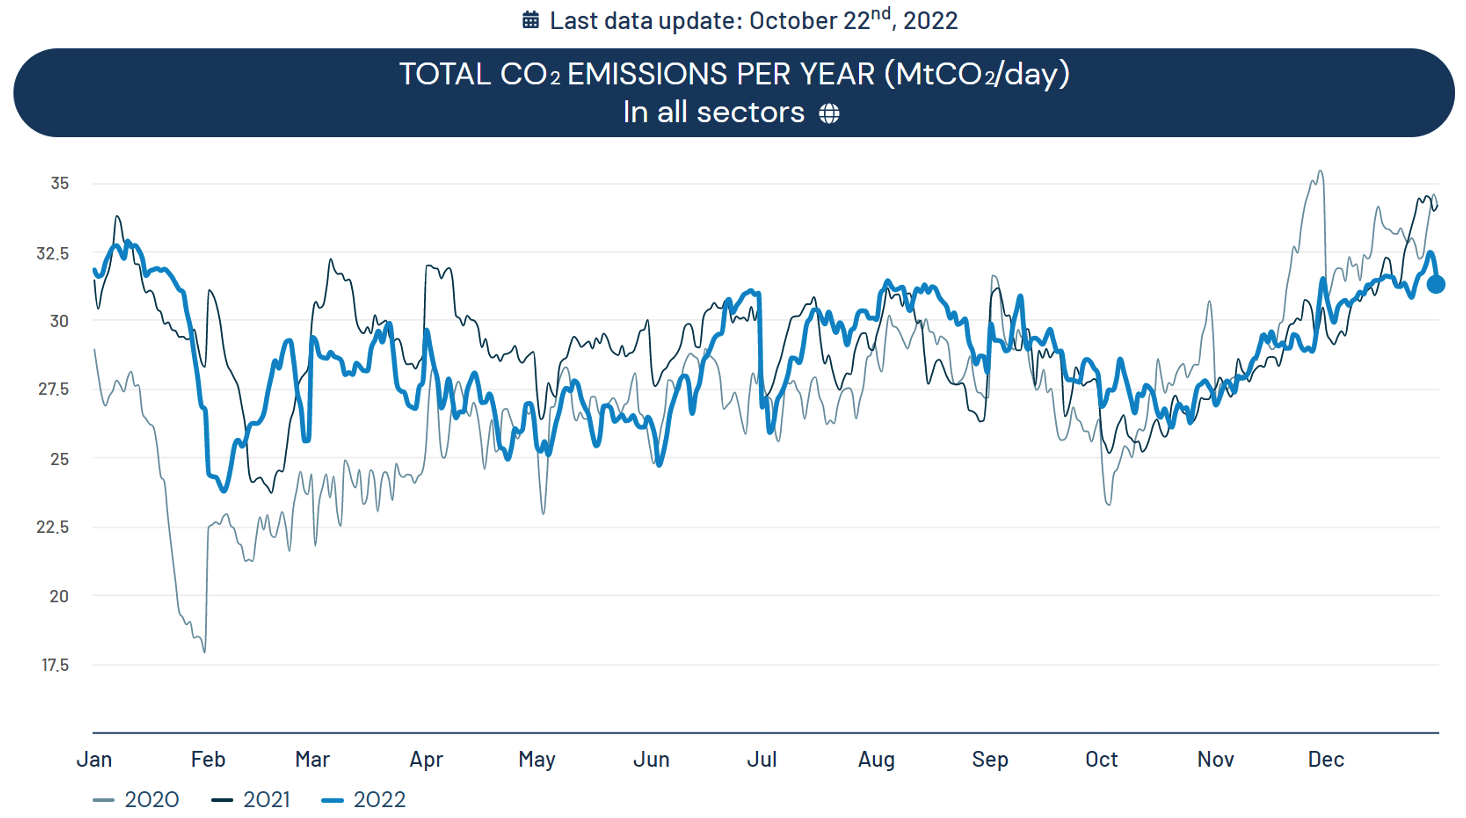
\includegraphics[width=\textwidth]{figures/total_carbon_emissions.png}
	\caption{Total Carbon Emissions across Investigated Sectors}
	\Description{} \label{fig:teaser}
\end{teaserfigure}

%%
%% This command processes the author and affiliation and title
%% information and builds the first part of the formatted document.
\maketitle


\section{Introduction}
Global warming, far from being a recent phenomenon, can be perceived from another
point as a persisting dilemma that continues to impact both anthropogenic development
and the natural ecosystem. The primary agent provoking global warming is
attributed to the emissions of greenhouse gases. Empirical studies confirm that
carbon dioxide holds the dubious distinction of being the most abundant greenhouse
gas in the atmosphere, contributing a staggering 72\% to global warming \cite{li2021-pricing}.

However, it is noteworthy to mention that China ranks as the preeminent
emitter of carbon dioxide on a global scale, discharging in excess of 6 billion
tonnes of carbon dioxide annually. Hence, addressing this crisis,
intrinsically connected to the existential fate of mankind, became a priority for
China. As a concrete commitment to this endeavor, President Xi Jinping, in
September 2020, proclaimed China's aim to "reach a peak in CO2 emissions by
2030 and accomplish carbon neutrality by 2060". The challenge of achieving
carbon neutrality is multifarious, necessitating a holistic approach,
encompassing policy, economy, culture, and technology. This paper opts to
focus on the forecasting of carbon emissions, a crucial foundational element for
strategic decision-making. Proficient predictions furnish invaluable data that
bolsters informed decision-making. Conversely, if the prognosis proves
inaccurate, ensuing plans may fall into the domain of impracticality \cite{-forecasting}.

The stakeholders who stand most directly impacted by these emissions include governments,
investors, and researchers. Government bodies, equipped with foresight into future
carbon emissions, can effectuate more meaningful change in climate policy, emergency
development, and global cooperation. Conversely, researchers and investors, informed
by predictive results, can more effectively design mechanisms such as the
Emissions Trading System, Carbon Pricing System, and related technologies. Consequently,
the act of forecasting carbon emissions carries significant implications for
subsequent research.

Since the year 2011, endeavors have been made to utilize logistic equations in
order to prognosticate China's carbon emissions \cite{meng2011-modeling}. At
present, the primary methodologies employed for the prediction of CO2 emissions
can be categorized into three principal clusters, specifically, statistical analysis
models, non-linear intelligent models, and grey prediction techniques \cite{gao2021-novel}.
Statistical models offer ease of application, yet they necessitate the collection
of ample historical data before the models can undergo training. Conversely, machine
learning frequently outperforms in forecasting relative to conventional statistical
methods.

This study implements the GNNs approach, presenting multiple advantages: Firstly,
GNNs are capable of effectively modelling spatial and temporal correlations. Secondly,
GNNs have the capacity to integrate additional contextual data, such as socio-economic
and policy factors. Thirdly, GNNs can yield an interpretable model structure,
thus enabling researchers to derive insights into the relationships between
various factors and their subsequent impact on carbon emissions\cite{alam2021-forecasting}.

At this juncture, GNNs have not been extensively explored in the context of
predicting carbon emissions. Hence, future research should pivot its focus
towards delving into the application of GNNs in carbon emissions forecasting. The
unique benefits offered by GNNs should be leveraged to construct models that are
both highly accurate and interpretable.

\section{Data Description}
Transitioning now to our research endeavor, the initial phase entailed data
acquisition from CarbonMonitor CHINA, a repository that chronicles the carbon emission
statistics for the past five years. We amassed more than 200 thousand data
points spanning from January 1, 2019, to December 31, 2022, systematically
segregating the data into 31 distinct states and five sectors respectively.

Subsequently, we performed a rudimentary data analysis, classified according
to temporality, sector, and state. A review of the past four years reveals that
carbon emissions peaked in the year 2021. Furthermore, a substantial variation
in carbon emissions was discerned across different sectors. Additionally, the
states of Hebei and Shandong emerged as the leading contributors to the nation's
carbon emissions.

\begin{figure}[ht]
	\centering
	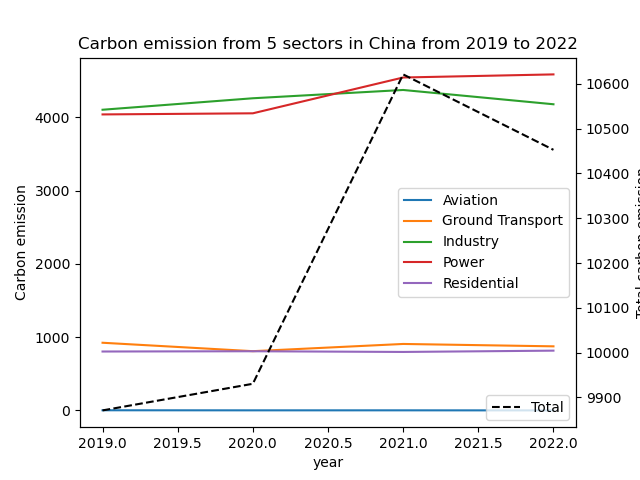
\includegraphics[width=0.4\textwidth]{figures/emissions_from_5_sectors.png}
	\caption{A graphical representation of emissions from five different sectors.}
	\label{fig:emissions_from_5_sectors}
\end{figure}

\begin{figure}[ht]
	\centering
	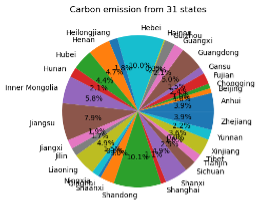
\includegraphics[width=0.4\textwidth]{figures/emissions_from_31_states.png}
	\caption{A graphical representation of emissions from 31 different states.}
	\label{fig:emissions_from_31_states}
\end{figure}

\section{Methodology}


In this section of the term paper, we systematically explore the technical aspects
of three distinct machine learning methodologies that are used in our study:
the Adaptive Graph Convolutional Recurrent Neural Network (AGCRN), Multi-Layer
Perceptron (MLP), and Fully Connected Long Short-Term Memory (FC-LSTM).

\subsection{Adaptive Graph Convolutional Recurrent Neural Network (AGCRN)}


Carbon emissions inherently form a complex, interconnected network due to their
origin from various sources and impacts on various regions. This network
extends both across different regions (spatial) and over time (temporal), which
makes AGCRN uniquely suited for carbon emissions prediction. During the
implementation, we mainly refer to the paper \cite{bai2020-adaptivea}.

AGCRN's GCN component efficiently captures the interplay between different regions,
considering how the carbon footprint in one region might influence and be
influenced by the emissions in other regions. Its RNN component focuses on the
temporal aspect, modeling how emissions evolve over time, including trends and
seasonality, which are common in environmental data. Hence, the AGCRN model
provides a comprehensive, holistic perspective in carbon emissions forecasting.

\begin{figure}[ht]
	\centering
	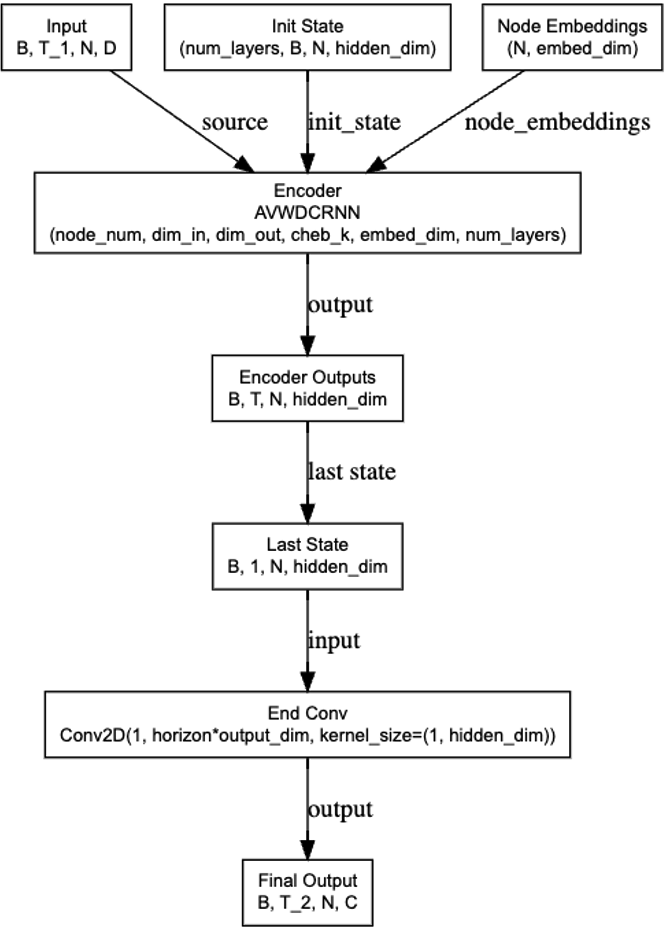
\includegraphics[width=0.4\textwidth]{figures/AGCRN_flow.png}
	\caption{AGCRN workflow.}
	\label{fig:AGCRN_flow}
\end{figure}

\subsection{Multi-Layer Perceptron (MLP)}


MLP is a fundamental form of artificial neural network, effective for capturing
non-linear relationships between inputs and outputs. When applied to carbon
emissions prediction, the MLP model can take into account various factors influencing
emissions, such as industrial production, energy consumption, population
density, and others. .

With its multiple layers and the capacity to learn complex mappings from inputs
to outputs, MLP can model the intricate interactions between these different
variables. Furthermore, the use of ReLU activation functions and dropout
regularization enhances the model's ability to generalize from the training
data, improving the robustness and reliability of predictions.

\begin{figure}[ht]
	\centering
	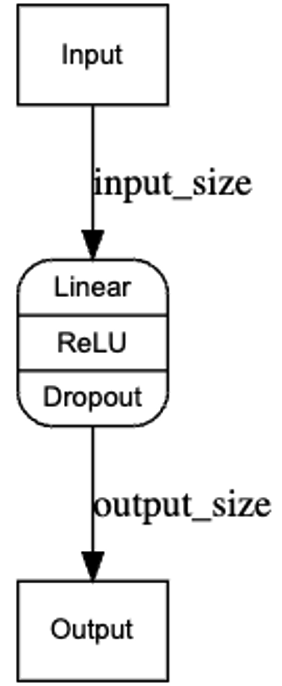
\includegraphics[width=0.15\textwidth]{figures/MLP_flow.png}
	\caption{MLP workflow.}
	\label{fig:MLP_flow}
\end{figure}

\subsection{Fully Connected Long Short-Term Memory (FC-LSTM)}


FC-LSTM is a recurrent neural network designed to capture long-term
dependencies in time-series data, which makes it ideal for carbon emissions prediction.
Carbon emissions data typically consist of time-series data, with various factors
influencing the emissions evolving over time. We mainly refer to the paper
\cite{tao2023-multiplea}.

The LSTM component, with its unique design of gating mechanisms, can
efficiently learn and recall past information when needed, making it adept at modeling
time-series data with long-term dependencies. These include identifying
increasing or decreasing trends in emissions over the years or understanding
seasonal variations. The fully connected layer helps in preserving the spatial
relationships between different provinces, thereby improving the model's
prediction capacity.

In essence, the FC-LSTM model's ability to consider past data and its capability
to model time dependencies, along with spatial relationships, makes it highly suitable
for predicting future carbon emissions.

\begin{figure}[ht]
	\centering
	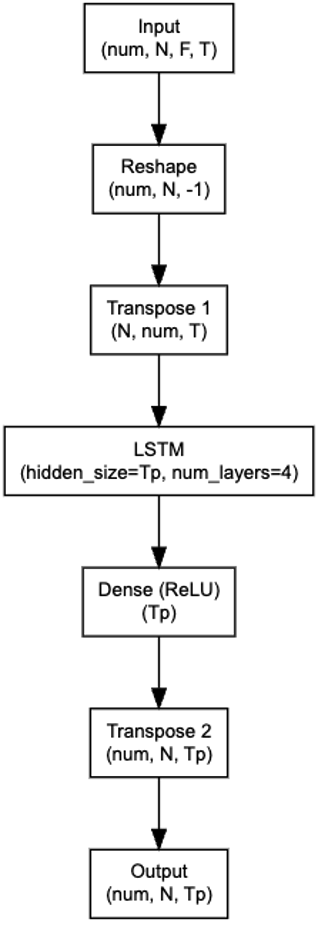
\includegraphics[width=0.15\textwidth]{figures/FC-LSTM_flow.png}
	\caption{FC-LSTM workflow.}
	\label{fig:FC-LSTM_flow}
\end{figure}

\section{Data Preprocessing}


The data for this study was sourced from
\href{https://cn.carbonmonitor.org/}{Carbon Monitor} which provides daily
carbon emissions data across different sectors for all 31 provinces in China. The
data spans from 2019 to 2022, resulting in a total of 1461 samples for each
province.

\subsection{Carbon Emissions Data Preprocessing}


Firstly, the raw data was retrieved from Carbon Monitor. For each province, the
daily carbon emissions from all sectors were summed up, providing a single
comprehensive measure of carbon emissions for each day. This process yielded a
time series data set for each province, where each data point represents the
total carbon emissions for a specific day.

\begin{algorithm}
	\caption{Carbon Emissions Data Preprocessing}
	\begin{algorithmic}
		[1] \For{each province} \For{each day from 2019 to 2022} \State Sum up carbon
		emissions from all sectors \EndFor \EndFor
	\end{algorithmic}
\end{algorithm}

\subsection{Province Adjacency Matrix Construction}


Next, a shapefile was utilized to calculate the adjacency of the provinces. If
two provinces share a border, they are considered adjacent, and the corresponding
entry in the adjacency matrix is set to 1; otherwise, it is set to 0. This adjacency
matrix serves as the preliminary graph structure, which will be further
refined during the training process of the Graph Neural Network (GNN) model.

\begin{algorithm}
	\caption{Construction of Province Adjacency Matrix}
	\begin{algorithmic}
		[1] \For{each pair of provinces} \If{they are adjacent} \State Set the corresponding
		adjacency matrix entry to 1 \Else \State Set the corresponding adjacency matrix
		entry to 0 \EndIf \EndFor
	\end{algorithmic}
\end{algorithm}

The preprocessing of the carbon emissions data, along with the construction of
the province adjacency matrix, serves as the foundation for the subsequent application
of GNNs for forecasting carbon emissions in China's provinces.

\section{Experiment}


In this section, we present the experiment of these three models, AGCRN, MLP
and FC-LSTM.

\subsection{Evaluation Metrics }
To compare the model performance, we implement MAE, MAPE and RMSE to measure
these three models.

\emph{MAE:} MAE measures the average absolute difference between the predicted
and actual carbon emissions. It evaluates the model's ability to make accurate
predictions.
\[
	MAE(y, \hat{y}) = \frac{1}{n}\sum_{i=1}^{n}|y_{i}- \hat{y}_{i}|
\]
\emph{MAPE:} MAPE measures the average absolute percentage difference between
the predicted and actual carbon emissions. It is used to evaluate the accuracy
of the model's predictions relative to the actual values.
\[
	MAPE(y, \hat{y}) = \frac{1}{n}\sum_{i=1}^{n}\frac{||y_{i}- \hat{y}_{i}||}{||y_{i}||}
\]

\emph{RMSE:} RMSE is the square root of the MSE and is used to measure the standard
deviation of the errors made by the model.
\[
	RMSE(y, \hat{y}) = \sqrt{\frac{1}{n}\sum_{i=1}^{n}(y_{i}- \hat{y}_{i})^{2}}
\]
\subsection{Simulation Results}
In the simulation section, the parameter settings are listed in Table.
\ref{Parameter settings }, we split the datasets into 70\% training data, 15\%
validation data and 15\% test data.

\begin{table}
	\caption{Parameter settings }
	\label{Parameter settings }
	\begin{tabular}{cl}
		\toprule Parameter/Setting    & Value  \\
		\midrule Tp                   & 1d     \\
		Tr                            & 10d    \\
		Loss function                 & L2Loss \\
		Optimizer                     & Adam   \\
		Percentage of training data   & 70\%   \\
		Percentage of validation data & 15\%   \\
		Percentage of test data       & 15\%   \\
		Epochs                        & 100    \\
		Number of runs                & 1      \\
		\bottomrule
	\end{tabular}
\end{table}

In Table. \ref{Average performance}, we exhibit the average performance
comparison of different approaches. As you can see, the AGCRN performs the
best in the three methods. MAE is 0.0151, MAPE is 2.7\% and RMSE is 0.0263.

\begin{table}
	\caption{Average performance comparison of different approaches.}
	\label{Average performance}
	\begin{tabular}{cccl}
		\toprule Method & MAE      & MAPE      & RMSE     \\
		\midrule AGCRN  & $0.0151$ & $2.7\%$   & $0.0263$ \\
		MLP             & $0.0699$ & $8.8\%$   & $0.1010$ \\
		FC-LSTM         & $0.5447$ & $412.7\%$ & $0.4984$ \\
		\bottomrule
	\end{tabular}
\end{table}

The AGCRN model outperformed the MLP and FC-LSTM models in our experiment, primarily
due to its ability to capture the complex spatiotemporal dependencies of carbon
emissions. The graph-based convolutional neural network structure of the AGCRN
model enables it to extract features from the spatial and temporal domains
simultaneously, resulting in more accurate predictions. In contrast, the MLP and
FC-LSTM models are traditional machine learning models that rely on linear regression
and LSTM networks, respectively, to forecast carbon emissions.

\subsection{Performance Evaluation }
In the experiment, we also visualize the prediction result and evaluate the
performance, as shown in Fig. \ref{fig:AGCRN} and Fig. \ref{fig:MLP}.

\begin{figure}[h]
	\centering
	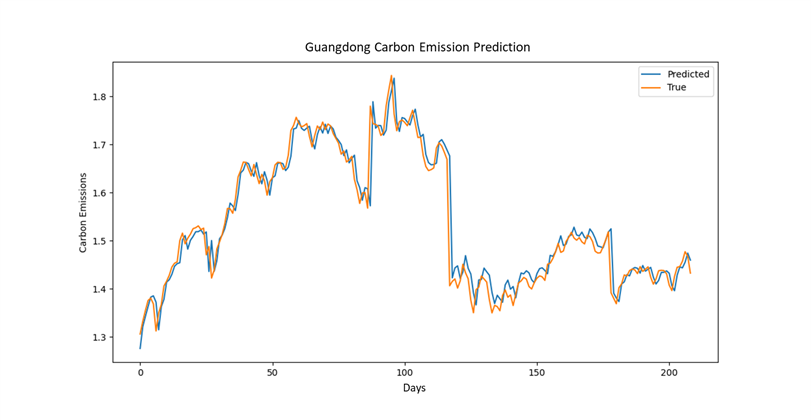
\includegraphics[width=\columnwidth]{figures/AGCRN.png}
	\caption{AGCRN.}
	\label{fig:AGCRN}
\end{figure}

\begin{figure}[h]
	\centering
	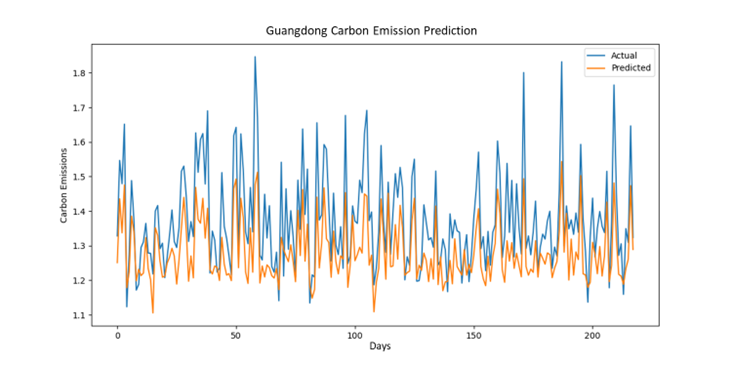
\includegraphics[width=\columnwidth]{figures/MLP.png}
	\caption{MLP.}
	\label{fig:MLP}
\end{figure}

From these two pictures of Guangdong carbon emission prediction, we can
apparently find that the AGCRN has better prediction results than MLP, which further
proves that the AGCRN method is more suitable for carbon emission prediction.

In conclusion, the AGCRN model's superior performance in predicting carbon
emissions can be attributed to its unique graph-based convolutional neural
network structure, which allows it to capture the intricate spatiotemporal dependencies
of carbon emissions. This study's findings offer valuable insights into the
development of more accurate and effective models for predicting carbon
emissions, which can inform policymakers and stakeholders in their efforts to reduce
carbon emissions and mitigate climate change.

\section{Conclusion and Future Work}


In this course project, we presented three models, AGCRN, MLP, and FC-LSTM,
for predicting the daily carbon emissions of 31 Chinese provinces using
historical data from January 1st, 2019 to December 31st, 2022. Our results
demonstrated that the AGCRN model outperformed the MLP and FC-LSTM models, indicating
its robustness in predicting carbon emissions accurately.

The findings of this project offer a new approach to enhance the precision of carbon
emission prediction. The AGCRN model's superior performance can be attributed
to its ability to capture the complex spatial and temporal dependencies of
carbon emissions. Our study provides valuable insights into the development of
more accurate and effective models for predicting carbon emissions, which can
inform policymakers and stakeholders in their efforts to reduce carbon
emissions and mitigate climate change.

\emph{Future work:} This project model can help carbon market stakeholders
grasp the future trend of the carbon market more accurately and provide a
reference for policymakers and investors in decision-making. However, the
quality and availability of the carbon emission data are low, which makes it hard
to improve the accuracy rapidly.

In future work, we can consider more factors to improve the accuracy of carbon
emission prediction such as weather, seasonality, and economic conditions. What’s
more, it is necessary to improve the computational complexity.

%%
%% The next two lines define the bibliography style to be used, and
%% the bibliography file.
\bibliographystyle{unsrtnat}
\bibliography{DSAA5020_Final_Report}


%%
%% If your work has an appendix, this is the place to put it.
\appendix
\section{Appendix}
\renewcommand{\thetable}{A.\arabic{table}}
\setcounter{table}{0}


\begin{table}[ht]
	\centering
	\caption{Contribution of each person in the project}
	\begin{tabularx}
		{\columnwidth}{|>{\centering\arraybackslash}m{2cm}|X|}
		\hline
		\textbf{Name} & \textbf{Tasks}                                                        \\
		\hline
		Xiao FANG     & Presenter, Background Investigation, FC-LSTM Training, Model Building \\
		\hline
		Hanyu GONG    & Presenter, Model Evaluation, MLP Training, Model Building             \\
		\hline
		Mingze GONG   & Presenter, Data Preprocessing, AGCRN Training, Model Building         \\
		\hline
	\end{tabularx}
	\label{table:contributions}
\end{table}

\end{document}
\endinput
%%
%% End of file `sample-authordraft.tex'.